
\chapter[ಭಾಗ -  2]{}\label{chap2}

\begin{center}
\rule{5cm}{1pt}\\[5pt]
{\Large\bfseries ಅಲಂಕಾರಿಕ ವಸ್ತುಗಳ ತಯಾರಿಕೆ }\\[3pt]
\rule{5cm}{1pt}
\end{center}
 
 \begin{itemize}
 \item ನಿರ್ದಿಷ್ಟ ಮಾನ ಆಕಾರಗಳು (6 ರೀತಿಯಲ್ಲಿ)
 \item  ಮೀನನ ರಚನೆ
 \item Flower for Rose
 \item Six point star
 \item ಮಾಘ ಮಾಲೆ
 \item ಹಡಗ ತಯಾರಿಕೆ
 \item ದ್ವಿಪಾದ ಹಡಗು
 \item wind mill
 \item ಟ್ರೇ
 \item ಕಪ್ 
 \item samurais Helmet
 \item  yakka-San.
  \end{itemize}
 
 \section*{ಓರಿಗಾಮಿಯಲ್ಲಿ ನಿರ್ದಿಷ್ಟ ಮಾನ ಆಕಾರಗಳು [Standard Shapes]}
 
 ಈಗ ಸಾವಿರಾರು ಕಾಗದದ ಮಾದರಿಗಳನ್ನು ತಯಾರಿಸುವುದನ್ನು ತಿಳಿದುಕೊಂಡಿದ್ದೇವೆ. ಈ ಕಾಗದ ಮಾದರಿಗಳನ್ನು ತಯಾರಿಸುವಾಗ ಅನೇಕ ಹಂತಗಳಲ್ಲಿ ಕಾಗದವನ್ನು ಮಡಚಬೇಕಾಗುತ್ತದೆ. ಹೀಗೆ ಮಡಚಬೇಕಾದರೆ, ಒಂದು ನಿರ್ದಿಷ್ಟ ಆಕಾರದ ಮಡಚುವಿಕೆಯನ್ನು ಪ್ರಾರಂಭದ ಹಂತದಲ್ಲಿ ಬಳಸುತೇವೆ. ಈ ರೀತಿಯ ಮಡಚುವಿಕೆಯನ್ನು "ನಿರ್ದಿಷ್ಟ ಮಾನ ಆಕಾರಗಳು" [Standard shapes] ಎಂದು ಕರೆಯುತ್ತೇವೆ. ಮುಖ್ಯವಾಗಿ `S' ನಿರ್ದಿಷ್ಟ ಮಾನ ಆಕಾರಗಳು ಇರುತ್ತವೆ. ಅವು ಒಂದಕ್ಕೊಂದು ಆಂತರಿಕವಾಗಿ ಸಂಬಂಧ ಹೊಂದಿರುತ್ತವೆ. ಅವು ಕೆಳಗಿನಂತೆ ಇರುತ್ತವೆ. 
  \begin{enumerate}
  \item[{\bf [1]}] \textbf{Waterbomb Base :} ಇದೊಂದು ಪ್ರಾರಂಭದ ನಿರ್ದಿಷ್ಟಮಾನ ಆಕಾರವಾಗಿದೆ. ಇದರ 5 ಬಿಂದುಗಳು ಅನೇಕ ನಕ್ಷೆಗಳಿಗೆ ಪರಿವರ್ತನ ಶೀಲ ಆಕಾರಗಳನ್ನು ಮಾಡುತ್ತವೆ. ಇದರಿಂದ "water bomb"ನ್ನು ತಯಾರಿಸಬಹುದು.

\medskip
  
  \item[{\bf [2]}] \textbf{Preliminary Base:} ಇದು ಅನೇಕ ನಿರ್ದಿಷ್ಟ ಮಾನ ಆಕಾರಗಳಿಗೆ ಪ್ರಾರಂಭದ ಹಂತವಾಗಿರುತ್ತದೆ. ಅಂದರೆ ಇದರಿಂದ "Bird Base" "Frog/lily Base" "paper crane", "Tato, Flopping Bird"  ಮುಂತಾದವುಗಳನ್ನು ತಯಾರಿಸಬಹುದು.  

\medskip
  
  \item[{\bf [3]}] \textbf{Frog/lily Base:} ಇದು ದಿಂದ ಪ್ರಾರಂಭವಾಗುತ್ತದೆ. ಅಂದರೆ ಈ ವಿಧಾನದಿಂದ ಮತ್ತು ಗಳನ್ನು ತಯಾರಿಸಬಹುದು.

\medskip
   
  \item[{\bf [4]}] \textbf{Bird  Base:} ಇದು ಯ ಪ್ರಾರಂಭದ ಹಂತವಾಗಿದೆ. ಇದರಿಂದ ಅನೇಕ ಪಕ್ಷಿಗಳನ್ನು/ಪ್ರಾಣಿಗಳನ್ನು ತಯಾರಿಸಬಹುದು. 
  
  \medskip
  
  \item[{\bf [5]}] \textbf{Fish Base:}  ಇದು ಅನೇಕ ಸಂಕೀರ್ಣ ಮಾದರಿಗಳ ತಯಾರಿಕೆಯಲ್ಲಿ ಪ್ರಾರಂಭದ ಹಂತವಾಗಿರುತ್ತದೆ. ಇದರಿಂದ "ಪಾರಂಪರಿಕ ಮೀನ್"ದ ಮಾದರಿಯನ್ನು ರಚಿಸಬಹುದು.
  
  \medskip
  
  \item[{\bf [6]}] \textbf{ಗಾಳಿಪಟ ಅಡಿಪಾಯ : Kite Base:} ಇದೊಂದು ಮುಖ್ಯವಾದ ಅಡಿಪಾಯವಾಗಿದೆ. ಇದರಿಂದ ವಿವಿಧ ರೀತಿಗಳಲ್ಲಿ ಕಾಗದವನ್ನು ಮಡಚಿ ವಿವಿಧ ರೀತಿಯ ಪಕ್ಷಿಗಳನ್ನು ತಯಾರಿಸಲು ಬರುತ್ತದೆ. 
\end{enumerate}

\medskip
\medskip

\begin{enumerate}
\item[{\bf [1]}] \textbf{ವಾಟರ್ ಬಾಂಬು ಅಡಿಪಾಯ  [Water bomb Base]}
\begin{figure}[H]
\centering{\includegraphics{src/figure/chap2/fig2-1a.eps}}
\end{figure}
\begin{figure}[H]
\centering{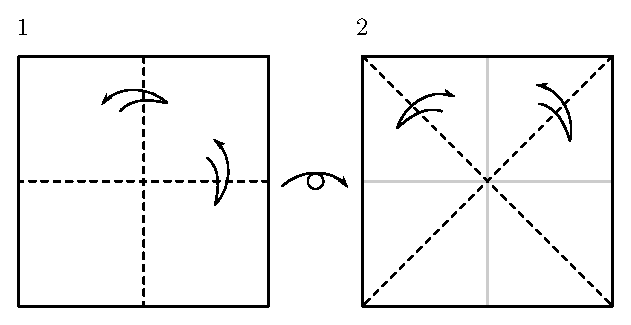
\includegraphics[scale=.85]{src/figure/chap2/fig2-1b.eps}}\\
\textbf{1. ಬಣ್ಣದ ಬದಿ ಮೇಲೆ ಇರುವಂತೆ ಚಿತ್ರದಲ್ಲಿ ತೋರಿಸಿದಂತೆ ಮಡಚಿ ತೆಗೆಯಬೇಕು.}\\
\textbf{2. ಕರ್ಣದ ಗುಂಟ ಮಡಚಿ ಬಿಚ್ಚಬೇಕು.}
\end{figure}
\begin{figure}[H]
\centering{\includegraphics[scale=.85]{src/figure/chap2/fig2-1c.eps}}
\end{figure}


\item[{\bf [2]}] \textbf{Preliminary Base: "ಪ್ರಾರಂಭಿಕ ಅಡಿಪಾಯ"}
ಈ ವಿಧಾನವನ್ನು ಪಕ್ಷಿಗಳ, ಕಪ್ಪೆ  ಮತ್ತು `ಲಿಲ್ಲಿ' ಹೂಗಳನ್ನು ತಯಾರಿಸಲು ಅಡಿಪಾಯವಾಗಿದೆ. ಇದು ಹೆಚ್ಚು ಸಾಮಾನ್ಯ ವಿಧಾನವಾಗಿದೆ. 
\begin{figure}[H]
\centering{\includegraphics[scale=.85]{src/figure/chap2/fig2-2.eps}}
\end{figure}

\noindent
\textbf{ಮಡಚುವ ಹಂತಗಳು :}
\begin{figure}[H]
\centering{\includegraphics[scale=.85]{src/figure/chap2/fig2-2a.eps}}
\end{figure}
\begin{figure}[H]
\centering{\includegraphics[scale=.85]{src/figure/chap2/fig2-2b.eps}}
\end{figure}

\item[{\bf [3]}]  \textbf{Frog/Lily Base :} ಇದು "Preliminary base" ವಿಧಾನದಿಂದ ಪ್ರಾರಂಭವಾಗುತ್ತದೆ.
\begin{figure}[H]
\centering{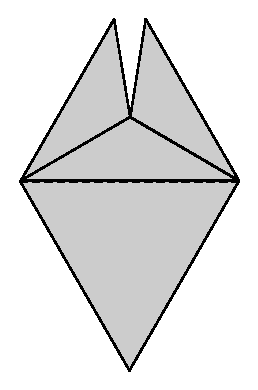
\includegraphics[scale=.85]{src/figure/chap2/fig2-3.eps}}
\end{figure}

ಅಂದರೆ, "Preliminary Base" ವಿಧಾನವು ಪೂರ್ಣಗೊಂಡ ನಂತರ ಈ ಮಡಚುವ ಹಂತಗಳು ಪ್ರಾರಂಭವಾಗುತ್ತವೆ.

ಇಲ್ಲಿ ಒಂದು ಬದಿಬಣ್ಣದ ಹಾಗೂ ಇನ್ನೊಂದು ಬದಿ ಬಿಳಿ ಬಣ್ಣವಿರುವ ಕಾಗದವನ್ನು ಚೌರಸ ಆಕಾರದಲ್ಲಿ ತೆಗೆದುಕೊಂಡು ಪ್ರಾರಂಭ ಮಾಡಬೇಕು.

\medskip
\noindent
\textbf{ಮಡಚುವ ಹಂತಗಳು :}
\begin{itemize}
\item[{\bf 1.}] \textbf{Preliminary Base ಮುಗಿದಾಗ ಬಣ್ಣದ ಭಾಗವು ಮೇಲೆ ಬರುತ್ತದೆ.}

\item[{\bf 2.}] \textbf{ಹಂತ 1ನ್ನು 180$^{\circ}$ ಕೋನ ಮಾಡಿ ತಿರುಗಿಸಬೇಕು. ತೆರೆದ ಭಾಗ ಮೇಲೆ ಬರುತ್ತದೆ.}
\begin{figure}[H]
\centering{\includegraphics{src/figure/chap2/fig2-3a.eps}}
\end{figure}

\item[{\bf 3.}] \textbf{ಒಂದು ಬದಿಯಲ್ಲಿ ಚಿತ್ರದಲ್ಲಿ ತೋರಿಸಿದಂತೆ ಮಡಚಬೇಕು. ಉಳಿದ ಭಾಗಗಳನ್ನು ಮಡಚಬೇಕು.}
\begin{figure}[H]
\centering{\includegraphics{src/figure/chap2/fig2-3b.eps}}
\end{figure}

\item[{\bf 4.}] \textbf{ಮೇಲಿನ ಪದರನ್ನು ಮಾತ್ರ ಮಧ್ಯದ ಗೆರೆಯಗೆ ಮಡಚಬೇಕು.}

\item[{\bf 5.}] \textbf{ದಳದ ಮಡಿಕೆ. ಮೇಲಿನ ಪದರನ್ನು ಪೂರ್ಣವಾಗಿ ಕೆಳಮುಖ ಮಡಚಬೇಕು ಮತ್ತು ಮಧ್ಯದ ಗೆರೆಗೆ ಬದಿಗಳನ್ನು ಮಡಚಬೇಕು. ಕೊನೆಗೆ ಉಬ್ಬು ಮಡಿಕೆ ಮಾಡಬೇಕು.}
\begin{figure}[H]
\centering{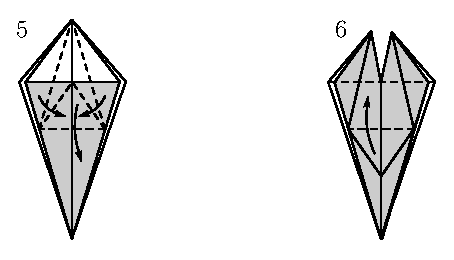
\includegraphics{src/figure/chap2/fig2-3c.eps}}
\end{figure}

\item[{\bf 6.}] \textbf{ದಳದ ಮಡಿಕೆಯನ್ನು ಮುಗಿಸಿ, ತಗ್ಗು ಮಡಿಕೆ ಮಾಡಿ ತ್ರಿಭುಜ ಆಕಾರದ ಭಾಗವನ್ನು ಮೇಲಕ್ಕೇ ಮಡಚಬೇಕು. ಮತ್ತು 4 ಮತ್ತು 6 ಹಂತಗಳನ್ನು ಉಳೀದ 3ಬದಿಗಳಲ್ಲಿ ಮಾಡಿ ಮುಗಿಸಬೇಕು.}

\item[{\bf 7.}] \textbf{ಈಗ Frog/Lily ಮಡಿಕೆ. ಪೂರ್ಣವಾಗಿದೆ.}
\begin{figure}[H]
\centering{\includegraphics[scale=.85]{src/figure/chap2/fig2-3d.eps}}
\end{figure}
\end{itemize}


\eject

\item[{\bf [4]}]  \textbf{ಪಕ್ಷಿ ಮಾದರಿ [Bird Base] ಮಡುಚುವಿಕೆ: ಪಕ್ಷಿ ಅಡಿಪಾಯ}
\begin{figure}[H]
\centering{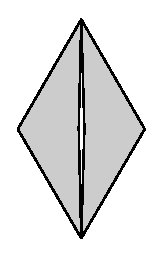
\includegraphics[scale=.95]{src/figure/chap2/fig2-4.eps}}\\
\end{figure}

ವಿವಿಧ ರೀತಿಯ ಪಕ್ಷಿಗಳನ್ನು ಹಾಗೂ ಪ್ರಾಣಿಗಳ ಮಾದರಿಗಳನ್ನು ತಯಾರಿಸಲು ಈ ಪಕ್ಷಿ ಮಾದರಿ ಮಡಿಕೆ ಉಪಯೋಗವಾಗುತ್ತದೆ. ಇದು "preliminary Base"ದಿಂದ ಮುಂದುವರಿಯುತ್ತವೆ. 
\begin{itemize}
\item[{\bf 1.}] \textbf{"Preliminary Base"ದಿಂದ ಮಡಿಕೆಯನ್ನು ಮುಂದುವರಿಸಬೇಕು.}
\begin{figure}[H]
\centering{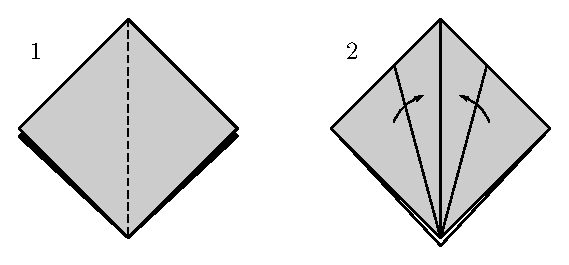
\includegraphics{src/figure/chap2/fig2-4a.eps}}
\end{figure}

\item[{\bf 2.}] \textbf{ಮೇಲಿನ ಪದರನ್ನು ಮಧ್ಯದ ಗೆರೆಗೆ ಮಡಚಬೇಕು.}

\item[{\bf 3.}] \textbf{ಮೇಲಿನ ತ್ರಿಭುಜವನ್ನು ಮಡಚಿರಿ.}
\begin{figure}[H]
\centering{\includegraphics[scale=0.85]{src/figure/chap2/fig2-4b.eps}}
\end{figure}

\item[{\bf 4.}] \textbf{ಮೇಲಿನ ಪದರನ್ನು ಮೇಲಕ್ಕೆ ಎತ್ತಿರಿ.}

\item[{\bf 5.}] \textbf{4ನೇ ಹಂತವು ಮುಂದುವರಿದಿದೆ. ಮಾದರಿಯು '3' ಆಯಾಮ ಆಗಿರುತ್ತದೆ. ಇರು:ದು ಗೆರೆಗಳ ಮೂಲಕ ಮೇಲಿನ ಪದರಗಳನ್ನು ಒಳಭಾಗದಲ್ಲಿ ಮಡಚಿರಿ.}
\begin{figure}[H]
\centering{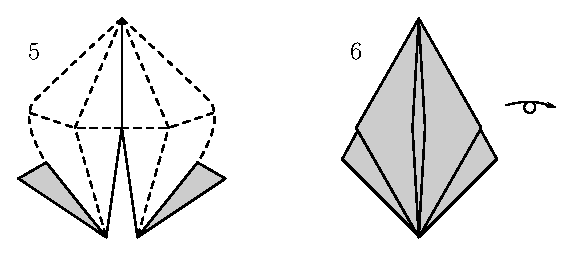
\includegraphics[scale=0.85]{src/figure/chap2/fig2-4c.eps}}
\end{figure}

\item[{\bf 6.}] \textbf{4ನೇ ಹಂತವು ಪೂರ್ಣವಾಗಿದ್ದು ಮಾದರಿಯು ಸಮತಟ್ಟಾವಾಗಿರುತ್ತದೆ. ಮಾದರಿಯನ್ನು ತಿರುವು ಮುರುವು ಮಾಡಿರಿ.}

\item[{\bf 7.}] \textbf{ಮತ್ತೊಂದು ಬದಿಯಲ್ಲಿ 2ರಿಂದ 6ರ ವರಗಿನ ಹಂತಗಳನ್ನು ಪೂನಾವರ್ತನೆ ಮಾಡಬೇಕು.}
\begin{figure}[H]
\centering{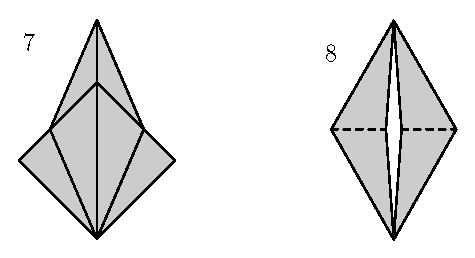
\includegraphics[scale=.8]{src/figure/chap2/fig2-4d.eps}}
\end{figure}

\item[{\bf 8.}] \textbf{ಪಕ್ಷಿ ಮಡಿಕೆ. (Bird Base) ಮುಗಿದಾಗ ಮಾದರಿ.}
\end{itemize}

\vfill\eject

\item[{\bf [5]}] \textbf{Fish Base : "ಮೀನು ಅಡಿಪಾಯ"}

ಒಂದು ಬದಿಬಣ್ಣದ ಇನ್ನೊಂದು ಬದಿ ಬಳಿ ಇರುವ ಚೌರಸ ಆಕಾರದ ಕಾಗದ ತೆಗೆದುಕೊಂಡು ಕೆಳಗಿನಂತೆ ಮಡಚಬೇಕು.
\begin{figure}[H]
\centering{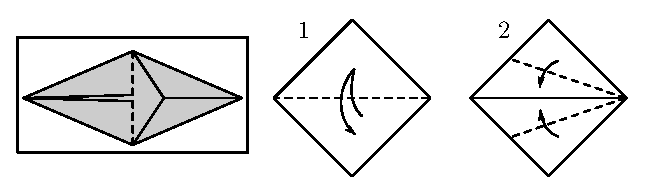
\includegraphics[scale=.85]{src/figure/chap2/fig2-5a.eps}}\\
\textbf{1. ಬಿಳಿಭಾಗ ಮೇಲೆ ಬರುವಂತೆ ಹಿಡಿದು ಒಂದು ಕರ್ಣದಗುಂಟ ಮಡಚಿ ತೆರೆಯಬೇಕು.}\\
\textbf{2. ನಂತರ ಕರ್ಣದ ಒಂದು ಬಿಂದುವಿನಿಂದ ಎರಡು ಶೃಂಗಬಿಂದುಗಳನ್ನು ಮಧ್ಯ ರೇಖೆಗೆ ಹೊಂದುವಂತೆ ಮಡಬೇಕು.}
\end{figure}
\begin{figure}[H]
\centering{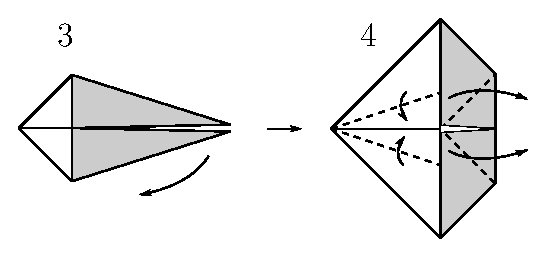
\includegraphics[scale=.85]{src/figure/chap2/fig2-5b.eps}}\\
\textbf{3. ಹಿಂಬದಿಗೆ ಅರ್ಧಭಾಗ ಉಬ್ಬು ಮಡಿಕೆ ಮಾಡಬೇಕು.}\\
\textbf{4. ಎರಡು ಬದಿಯಲ್ಲಿ 'Squash Fold' ಮಾಡಬೇಕು.}
\end{figure}
\begin{figure}[H]
\centering{\includegraphics[scale=.85]{src/figure/chap2/fig2-5c.eps}}\\
\textbf{5. ಹಿಂದಿನ ಪದರನ್ನು ಹಿಂಬದಿಗೆ ಉಬ್ಬು ಮಡಿಕೆ ಮಾಡಬೇಕು. }\\
\textbf{6. 'Fish Base' ಮಾದರಿ}
\end{figure}

\eject

\item[{\bf [6]}] \textbf{ಗಾಳಿಪಟ ಅಡಿಪಾಯ : [Kite Base]}

ಒಂದು ಬದಿ ದಟ್ಟಬಣ್ಣ ಇನ್ನೊಂದು ಬದಿ ಬಿಳಿ ಅಥವಾ ತೆಳುಬಣ್ಣದ ಚೌಕಾಕಾರದ ಹಾಳೆಯಿಂದ ಕೆಳಗಿನಂತೆ ಮಡಚಿ ಗಾಳಿಪಟ ಅಡಿಪಾಯವನ್ನು ಮಾಡಬಹುದು. 

\noindent
\textbf{ಮಡಚುವ ಹಂತಗಳು :}
\begin{figure}[H]
\centering{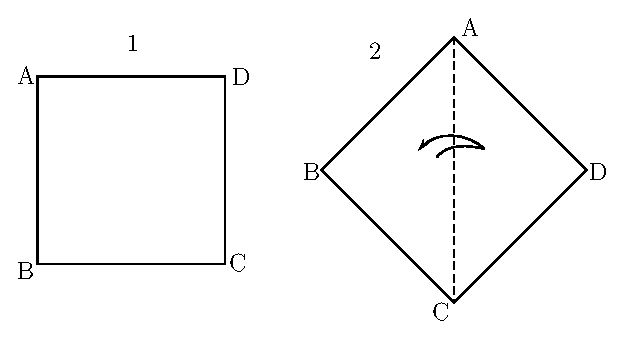
\includegraphics[scale=.85]{src/figure/chap2/fig2-6a.eps}}\\
\textbf{1. ಬಿಳಿ ಅಥವಾ ತೆಳುಬಣ್ಣದ ಬದಿ (ಮೈ) ಮೇಲೆ ಬರುವಂತೆ ಹಿಡಿಯಬೇಕು.}\\
\textbf{2. AC ಕರ್ಣದ ಗುಂಟ ಮಡಚಿ ನಂತರ ಬಿಚ್ಚಬೇಕು.}
\end{figure}
\begin{figure}[H]
\centering{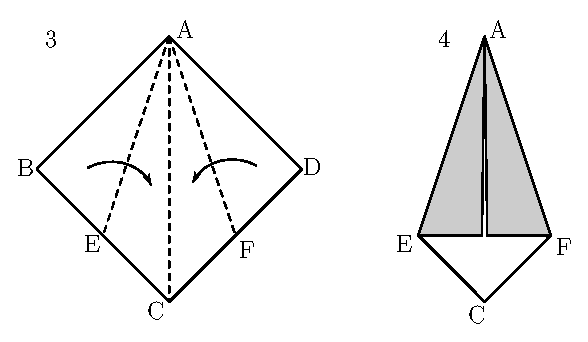
\includegraphics[scale=.85]{src/figure/chap2/fig2-6b.eps}}\\
\textbf{3. AB ಮತ್ತು AD ಬಾಹುಗಳನ್ನು  AC ಕರ್ಣಕ್ಕೆ ಸರಿಯಾಗಿ ಹೊಂದುವಂತೆ ಮಡಚಬೇಕು.}\\
\textbf{4. ಗಾಳಿಪಟ ಅಡಿಪಾಯ [Kite Base] ತಯಾರಾಯಿತು. ಈ 4 ಹಂತಗಳಿಂದ ಮುಂದುವರಿಸಿ ಅನೇಕ ಪಕ್ಷಿಗಳನ್ನು ತಯಾರಿಸಬಹುದು.}
\end{figure}
\end{enumerate}

\section*{ಅಲಂಕಾರಿಕ ವಸ್ತುಗಳ ಮಾದರಿಗಳ ತಯಾರಿಕೆ}

ಗಾಳಿಪಟ ಅಡಿಪಾಯವನ್ನು ಮುಂದುವರಿಸಿ ಈ ಮಾದರಿಯನ್ನು ಕೆಳಗಿನಂತೆ ತಯಾರಿಸಬಹುದು.
\begin{figure}[H]
\centering{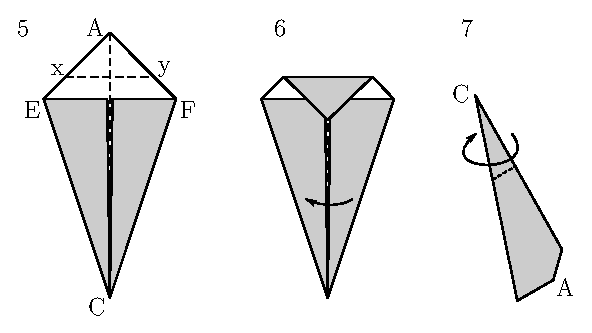
\includegraphics[scale=.85]{src/figure/chap2/fig2-6c.eps}}\\
\textbf{5. xy ಗೆರೆಯ ಗುಂಟ A ಬಿಂದುವನ್ನು ಮುಂದೆ ಮಡಿಚಬೇಕು.}\\
\textbf{6. AC ಕರ್ಣದ ಗುಂಟ ಒಳಮುಖವಾಗಿ ಮಡಚಬೇಕು.}\\
\textbf{7. C ಬಿಂದು ACಗೆ ಲಂಬವಾಗಿರುವಂತೆ ಮಡಚಬೇಕು.}
\end{figure}
\begin{figure}[H]
\centering{\includegraphics[scale=.85]{src/figure/chap2/fig2-6d.eps}}\\
\textbf{8. ಎರಡು ಜಾಗೆಗಳಲ್ಲಿ ಗೆರೆಗಳ ಗುಂಟ ಮಡಚಬೇಕು.}
\end{figure}

"ಗಾಳಿಪಟ ಅಡಿಪಾಯ"ವನ್ನು ಮುಂದುವರಿಸಿ ಈ ಮಾದರಿಯನ್ನು ಕೆಳಗಿನಂತೆ ತಯಾರಿಸಬೇಕು.
\begin{figure}[H]
\centering{\includegraphics[scale=.85]{src/figure/chap2/fig2-6e.eps}}
\end{figure}
\begin{figure}[H]
\centering{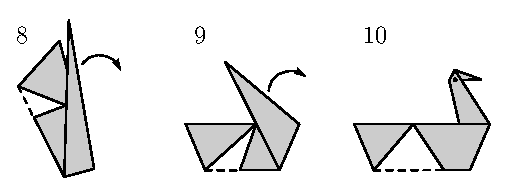
\includegraphics[scale=.85]{src/figure/chap2/fig2-6f.eps}}
\end{figure}

ಗಾಳಿಪಟ ಅಡಿಪಾಯ [Kite base] ಉಪಯೋಗಿಸಿ ಈ ಮಾದರಿಯನ್ನು ಕೆಳಗಿನಂತೆ ತಯಾರಿಸಬಹುದು.
\begin{figure}[H]
\centering{\includegraphics[scale=.85]{src/figure/chap2/fig2-6g.eps}}
\end{figure}
\begin{figure}[H]
\centering{\includegraphics[scale=.85]{src/figure/chap2/fig2-6h.eps}}
\end{figure}

ಗಾಳಿಪಟ ಅಡಿಪಾಯ [Kite base]ದ ಸಹಾಯದಿಂದ ಕೆಳಗಿನಂತೆ ಮಡಚಿ ಪಕ್ಷಿಯ ಮಾದರಿಯನ್ನು ತಯಾರಿಸುವುದು. 
\begin{figure}[H]
\centering{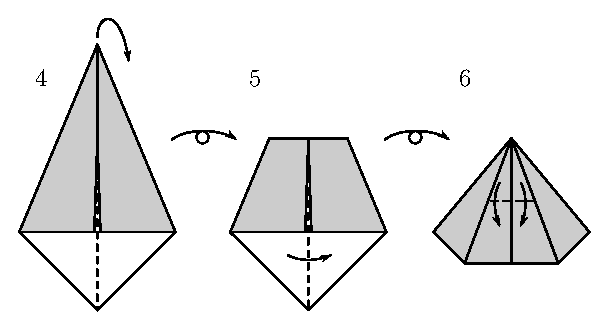
\includegraphics[scale=.85]{src/figure/chap2/fig2-6i.eps}}
\end{figure}
\begin{figure}[H]
\centering{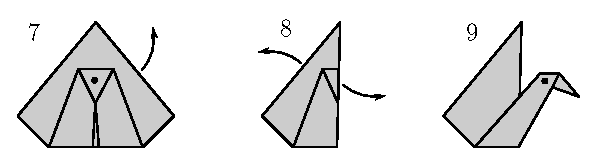
\includegraphics[scale=.85]{src/figure/chap2/fig2-6j.eps}}
\end{figure}


\medskip
\noindent
\textbf{ಮೀನು [Fish]}
\begin{figure}[H]
\centering{\includegraphics[scale=.85]{src/figure/chap2/fig2-7.eps}}
\end{figure}

\eject
\noindent
\textbf{ಮಡಚುವ ಹಂತಗಳು :}
\begin{figure}[H]
\centering{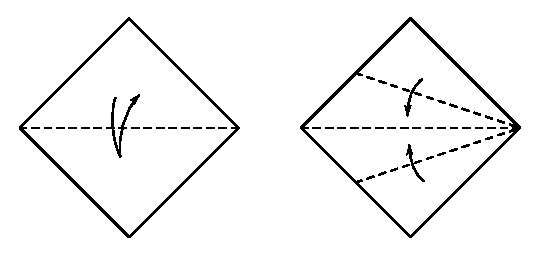
\includegraphics[scale=.85]{src/figure/chap2/fig2-7a.eps}}\\
\textbf{1. ಬಿಳಿಭಾಗವು ಮೇಲೆ ಬರುವಂತೆ ಹಿಡಿದು ಕರ್ಣದ ಗುಂಟ ಮಡಚಿ ಬಿಚ್ಚಬೇಕು.}\\
\textbf{2. ಅಡ್ಡ ಗೆರೆಯ ಮೇಲಿನ ಮತ್ತು ಕೆಳಗಿನ ಶೃಂಗಗಳನ್ನು ಮಧ್ಯ ಗೆರೆಗೆ ಹೊಂದುವಂತೆ ಮಡಚಬೇಕು.}
\end{figure}
\begin{figure}[H]
\centering{
\includegraphics[scale=.85]{src/figure/chap2/fig2-7b.eps}}\\
\textbf{3. ಬಲಭಾಗದ ಶೃಂಗವನ್ನು ಹಿಂದಕ್ಕೆ ಅರ್ಧಭಾಗಕ್ಕೆ ಸರಿಯಾಗುವಂತೆ ಮಡಚಬೇಕು.}\\
\textbf{4. ಚಿತ್ರದಲ್ಲಿ ತೋರಿಸಿದಂತೆ ಎರಡು ಬದಿಯನ್ನು ಮಧ್ಯ ರೇಖೆಗೆ ಹೊಂದುವಂತೆ ಮಡಚಿ. ಹಿಂದೆ ಹಾಗೂ ಮುಂದಿನ ಭಾಗಗಳನ್ನು ಮೊದಲಿನಂತೆ ಮಾಡಬೇಕು.}
\end{figure}
\begin{figure}[H]
\centering{\includegraphics[scale=.85]{src/figure/chap2/fig2-7c.eps}}\\
\textbf{6. ಹಿಂದಿನ ಪದರನ್ನು ಹಿಂದಕ್ಕೆ ಉಬ್ಬು ಮಡಿಕೆ ಮಾಡಬೇಕು.}
\end{figure}
\begin{figure}[H]
\centering{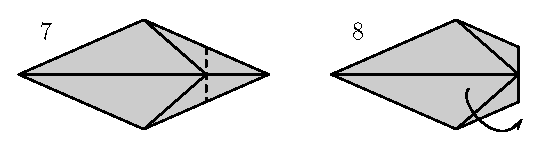
\includegraphics[scale=.85]{src/figure/chap2/fig2-7d.eps}}\\
\textbf{7. ಉಬ್ಬು ಮಡಿಕೆಯನ್ನು (ಗೆರೆಯ ಗುಂಟ) ಹಿಂಬದಿಗೆ ಮಾಡಬೇಕು. ಇದು "Fish base" ಆಗಿದೆ.}\\
\textbf{8. ಅರ್ಧಕ್ಕೆ ಉಬ್ಬು ಮಡಿಕೆ ಮಾಡಬೇಕು.}
\end{figure}
\begin{figure}[H]
\centering{\includegraphics[scale=.85]{src/figure/chap2/fig2-7e.eps}}\\
\textbf{9. ಹಕ್ಕಿಗಳನ್ನು ಕೆಳಕ್ಕೆ ಮಡಚಬೇಕು.}\\
\textbf{10. ಗೆರೆಯಗುಂಟ ಹಿಂಬದಿಗೆ ಮಡಚಬೇಕು.}
\end{figure}
\begin{figure}[H]
\centering{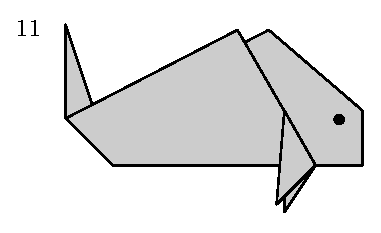
\includegraphics[scale=.85]{src/figure/chap2/fig2-7f.eps}}\\
\textbf{11. "ಮೀನ್‌ನ ಮಾದರಿ" Fish Model}
\end{figure}

\medskip
\noindent
\textbf{Flower for Rose}
\begin{figure}[H]
\centering{\includegraphics[scale=.85]{src/figure/chap2/fig2-8.eps}}
\end{figure}

\noindent
\textbf{ಮಡಚುವ ಹಂತಗಳು :}
\begin{figure}[H]
\centering{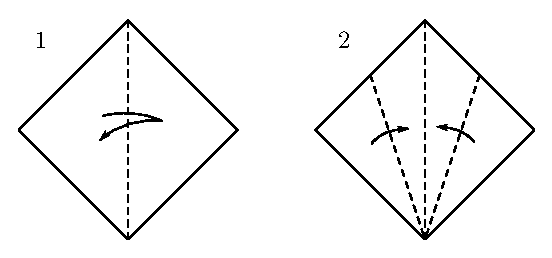
\includegraphics[scale=.85]{src/figure/chap2/fig2-8a.eps}}\\
\textbf{1. ಚೌರಸದ ಬಿಳಿಭಾಗವು ಮೇಲೆ ಇರುವಂತೆ ಒಂದು ಕರ್ಣದ ಗುಂಟ ಮಡಚಿ ಬಿಚ್ಚಬೇಕು.}\\
\textbf{2. ಹಂತ 1ರಲ್ಲಿ ಮಾಡಿದ ಗೆರೆಯ ಗುಂಟ ಎರಡು ಬದಿಗಳನ್ನು ಮಡಚಿ ಬಿಚ್ಚಬೇಕು.}
\end{figure}
\begin{figure}[H]
\centering{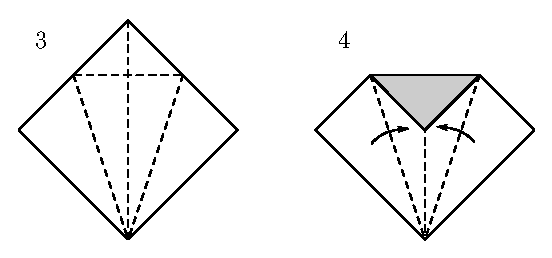
\includegraphics[scale=.85]{src/figure/chap2/fig2-8b.eps}}\\
\textbf{3. ಹಂತ 2ರಲ್ಲಿ ಮಾಡಿದ ಗೆರೆಗಳಿಗೆ ಹೊಂದಿಕೊಂಡು ಮೇಲಿನ ತುದಿಯನ್ನು ಕೆಳಮುಖವಾಗಿ ಮಡಚಬೇಕು.}\\
\textbf{4. ಹಂತ 3ರಲ್ಲಿ ಮಾಡಿದ ಗೆರೆಯ ಗುಳ ಎರಡು ಬದಿಗಳಲ್ಲಿ ಮಡಚಬೇಕು.}
\end{figure}
\begin{figure}[H]
\centering{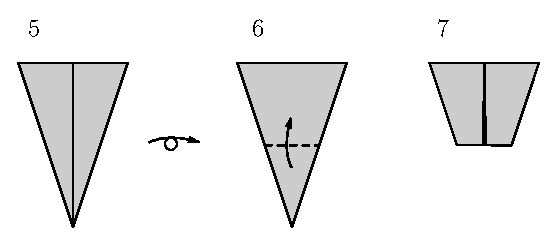
\includegraphics[scale=.85]{src/figure/chap2/fig2-8c.eps}}\\
\textbf{5. ಇದನ್ನು ತಿರುಗಿಸಬೇಕು.}\\
\textbf{6. ಕೆಳಮೂಲೆಯನ್ನು ಮೇಲಿನ ಭಾಗಕ್ಕೆ ತಾಗುವಂತೆ ಮಡಚಬೇಕು.}\\
\textbf{7. ಈಗ ಒಂದು ಮಾದರಿ ತಯಾರಾಯಿತು. ಇನ್ನು ಇಂತಹ 5 ಮಾದರಿಗಳನ್ನು ತಯಾರಿಸಬೇಕು.}
\end{figure}
\begin{figure}[H]
\centering{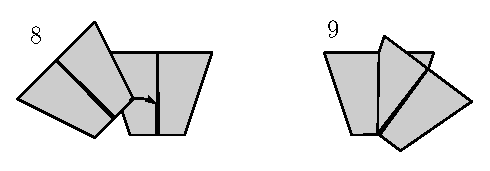
\includegraphics[scale=.85]{src/figure/chap2/fig2-8cc.eps}}\\
\textbf{8. ಚಿತ್ರದಲ್ಲಿ ಬಾಣದ ಗುರುತಿನ ಮಾರ್ಗದಲ್ಲಿ ಎರಡು ಮಾದರಿಗಳನ್ನು ಸೇರಿಸಬೇಕು.}\\
\textbf{9. ಎರಡು ಮಾದರಿಗಳನ್ನು ಜೋಡಿಸಿದಾಗ ಸಿಗುವ ವ್ಯವಸ್ಥೆ ಕೊನೆಯದಾಗಿ ಎಲ್ಲ ಮಾದರಿಗಳನ್ನು (Units) ಜೊಡಿಸಿದಾಗ, ನಮಗೆ "Flower for Rose" ದೊರಕುತ್ತದೆ.}
\end{figure}
\begin{figure}[H]
\centering{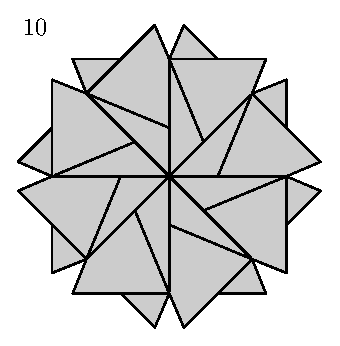
\includegraphics[scale=.85]{src/figure/chap2/fig2-8d.eps}}
\end{figure}

\medskip
\noindent
\textbf{6. ಶೃಂಗ ಬಿಂದುಗಳುಳ್ಳ ನಕ್ಷತ್ರ [Six Point Star]}

\noindent
\textbf{ಮಡಚುವ ಹಂತಗಳು :} 6 ಶೃಂಗ ಬಿಂದುಗಳುಳ್ಳ ನಕ್ಷತ್ರವನ್ನು ತಯಾರಿಸಲು ಎರಡು ಬೇರೆ\break ಬೇರೆ ಬಣ್ಣಗಳ ಕಾಗದವನ್ನು ತೆಗೆದುಕೊಂಡು ಒಂದು ಬಣ್ನದ 3 ಹಾಗೂ ಇನ್ನೊಂದು ಬಣ್ಣದ 3 ಪ್ರಾರಂಭಿಕ ಮಡಿಕೆಗಳನ್ನು ತಯಾರಿಸಬೇಕು. ನಂತರ ಅವುಗಳನ್ನು ಜೋಡಿಸಿದಾಗ 6. ಶೃಂಗ ಬಿಂದುಗಳುಳ್ಳ ನಕ್ಷತ್ರವು ತಯಾರಾಗುತ್ತದೆ. 
\begin{figure}[H]
\centering{\includegraphics[scale=.85]{src/figure/chap2/fig2-9.eps}}
\end{figure}

ಪ್ರಾರಂಭಿಕ ಮಡಿಕೆಯನ್ನು ತಯಾರಿಸಲು ಒಂದು ಬಣ್ಣದ (ಕೆಂಪು) ಚೌರಸ ಆಕಾರದ ಕಾಗದವನ್ನು ಕೆಳಗಿನಂತೆ ಮಡಚಬೇಕು.
\begin{figure}[H]
\centering{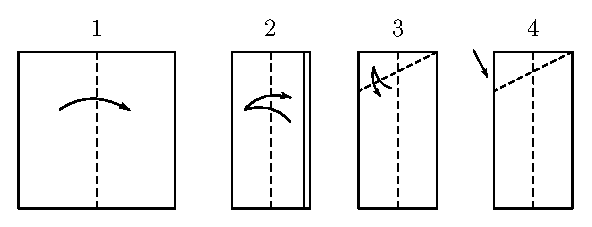
\includegraphics[scale=.85]{src/figure/chap2/fig2-9a.eps}}
\end{figure}
\begin{figure}[H]
\centering{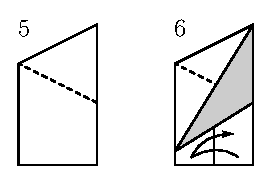
\includegraphics[scale=.85]{src/figure/chap2/fig2-9b.eps}}\\
\textbf{ಈ 6 ಹಂತಗಳಲ್ಲಿ 3 ಕೆಂಪು ಮತ್ತು 3 ಹಸಿರು ಕಾಗದ ಮಡಿಕೆಗಳನ್ನು ಮಾಡಿಕೊಂಡು ಕೆಳಗಿನಂತೆ ಬೇರೆ ಬೇರೆ ಹಂತಗಳಲ್ಲಿ ಜೋಡಿಸಬೇಕು.}
\end{figure}
 
 \noindent
 \textbf{ಜೋಡಣೆಯ ಹಂತಗಳು :}
 \begin{figure}[H]
\centering{\includegraphics[scale=.85]{src/figure/chap2/fig2-9c.eps}}\\
\textbf{1. ಬೇರೆ ಬೇರೆ ಬಣ್ಣಗಳ ಎರಡು ಘಟಕಗಳನ್ನು ಚಿತ್ರದಲ್ಲಿ ತೋರಿಸಿದಂತೆ ಜೋಡಿಸಬೇಕು.}\\
\textbf{2. ಈಗ 3ನೇ ಘಟಕವನ್ನು ಚಿತ್ರದಲ್ಲಿ ತೋರಿಸಿದಂತೆ ಜೋಡಿಸಬೇಕು.}
\end{figure}
 \begin{figure}[H]
\centering{\includegraphics[scale=.85]{src/figure/chap2/fig2-9d.eps}}\\
\textbf{3. ಹೀಗೆ ಒಂದರ ನಂತರ ಒಂದು ಬೇರೆ ಬೇರೆ ಬಣ್ಣಗಳ ಘಟಕಗಳನ್ನು ಪೂರ್ಣವಾಗಿ ಜೋಡಿಸಬೇಕು.}\\
\textbf{4. ಈ ಪೂರ್ಣ ಪ್ರಮಾಣದಲ್ಲಿ 6-ಶೃಂಗಗಳುಳ್ಳ ನಕ್ಷತ್ರದ ಮಾದರಿ ತಯಾರಾಗುತ್ತದೆ.}
\end{figure}

\noindent
\textbf{ಮೇಘು ಮಾಲೆ [WREATH] :}   

ಇದನ್ನು ಅಲಂಕಾರಿಕ ವಸ್ತುವಾಗಿ ಬಳಸುತ್ತಾರೆ. ಇದನ್ನು ಅಂಟು ಹಚ್ಚದೆ ಕೇವಲ ಜೋಡಣೆಯಿಂದ ಬಲಯುತವಾಗಿ ತಯಾರಿಸುತ್ತಾರೆ. ಇದು ಹೆಚ್ಚು ಅವಧಿಯವರಗೆ ಬಾಳಿಕೆ ಬರುತ್ತದೆ.
\begin{figure}[H]
\centering{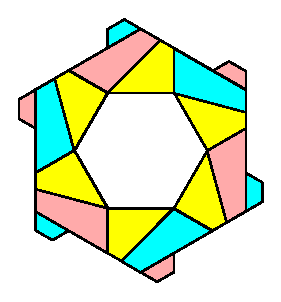
\includegraphics[scale=.95]{src/figure/chap2/fig2-10.eps}}
\end{figure}

\noindent
\textbf{ಮಡಚುವ ವಿಧಾನಗಳು :} ಒಂದು ಮೇಲ್ಮೈಯ ಬಣ್ಣದ ಹಾಗೂ ಮತ್ತೆಂದು ಭಾಗ ಬಿಳಿ ಇರುವ ಬೇರೆ ಬೇರೆ ಬಣ್ಣಗಳ ಚೌರಸ ಆಕಾರದ ಕಾಗದಗಳನ್ನು ತೆಗೆದುಕೊಳ್ಳಬೇಕು. ಇಲ್ಲಿ ಎರಡು ಬಣ್ಣಗಳ (ಕೆಂಪು ಮತ್ತು ನೀಲಿ) ಕಾಗದಗಳನ್ನು ತೆಗೆದುಕೊಂಡು ಒಂದು ಬಣ್ಣದ (ಕೆಂಪು) 3 ಹಾಗೂ ಇನ್ನೊಂದು ಬಣ್ಣದ (ನೀಲಿ) 3 ಹೀಗೆ ಒಟ್ಟು 6 ಭಾಗಗಳನ್ನು (Units) ತಯಾರಿಸಬೇಕು.

\noindent
\textbf{ಒಂದು ಭಾಗ (Unit)ನನ್ನು ತಯಾರಿಸುವುದು :}
\begin{figure}[H]
\centering{\includegraphics[scale=.85]{src/figure/chap2/fig2-10a.eps}}\\
\textbf{1. ಬಿಳಿಭಾಗ ಮೇಲೆ ಬರುವಂತೆ ಹಿಡಿದು ಲಂಬವಾಗಿ ಮಡಚಿ ತೆಗೆಯಬೇಕು.}\\
\textbf{2. ಪುಸ್ತಕ ಮಡಿಕೆ ಮಾಡಿ ಬಿಚ್ಚಬೇಕು.}\\
\textbf{3. ಬಲಭಾಗದ ಶೃಂಗಭಾಗ ಅಡ್ಡ ಗೆರೆಯ ಮೇಲೆ ಬರುವಂತೆ ಮಡಚಿ ಬಿಚ್ಚಬೇಕು.}
\end{figure}
\begin{figure}[H]
\centering{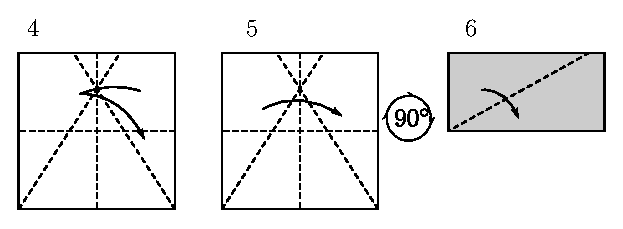
\includegraphics[scale=.85]{src/figure/chap2/fig2-10b.eps}}\\
\textbf{4. ಹಂತ 3ರಂತೆ ಎಡಭಾಗದಲ್ಲಿ ಮಾಡಬೇಕು.}\\
\textbf{5. 1ನೇ ಹಂತದಲ್ಲಿಯ ಗೆರೆಯ ಗುಂಟ ಮಡಚಬೇಕು.}\\
\textbf{6. 90$^{\circ}$ ಪ್ರದಕ್ಷೀಣಿಯವಾಗಿ ತಿರುಗಿಸಿ ಚಿತ್ರದಲ್ಲಿ ತೋರಿಸಿದಂತೆ ಗೆರೆಯ ಗುಂಟ ಒಳಭಾಗದಲ್ಲಿ ಮಡಚಬೇಕು. }
\end{figure}
\begin{figure}[H]
\centering{\includegraphics[scale=.85]{src/figure/chap2/fig2-10c.eps}}\\
\textbf{7. ಮೇಲಿನ ಶೃಂಗದಲ್ಲಿ ಒಳಭಾಗದಲ್ಲಿ ಮಡಚಬೇಕು. ಈಗ 1 ಭಾಗ (Unit) ತಯಾರಾಗುತ್ತದೆ. ಹೀಗೆ ಇನ್ನು 5 ಭಾಗಗಳನ್ನು ತಯಾರಿಸಬೇಕು.}\\
\textbf{8. ಬೇರೆ ಬೇರೆ ಬಣ್ಣಗಳ ಎರಡು ಭಾಗಗಳನ್ನು (Units) ಚಿತ್ರದಲ್ಲಿ ತೋರಿಸಿದಂತೆ ಒಂದರ ಒಳಗೆ ಒಂದನ್ನು ಸೇರಿಸಬೇಕು. ಹಾಗೂ ಒಂದರ ನಂತರ ಒಂದು ಬಣ್ಣದ ಭಾಗಗಳನ್ನು ಸೇರಿಸಿ ಪೂರ್ಣವಾಗಿ ಮೇಫು ಮಾಲೆಯನ್ನು ತಯಾರಿಸಬೇಕು.}
\end{figure}

\noindent
\textbf{ಹಡಗು [Boat] ಮಾದರಿ ತಯಾರಿಕೆ}

ಒಂದು ಮೇಲ್ಮೈ ಬಣ್ನದ ಮತ್ತು ಮತ್ತೊಂದು ಮೇಲ್ಮೈ ಬಿಳಿ ಅಥವಾ ತೇಳು ಬಣ್ಣದ ಒಂದು $A_4$ ಅಳತೆಯ ಕಾಗದಿಂದ ಕೆಳಗಿನಂತೆ ಮಡಚಿ ಹಡಗುವನ್ನು ತಯಾರಿಸುತ್ತಾರೆ. 

\noindent
\textbf{ಮಡಚುವ ಹಂತಗಳು :}
\begin{figure}[H]
\centering{\includegraphics[scale=.85]{src/figure/chap2/fig2-11a.eps}}\\
\textbf{1. ಬಿಳಿ ಅಥವಾ ತೇಳು ಬಣ್ಣದ ಮೈ ಮೇಲೆ ಇರುವಂತೆ ಪುಸ್ತಕ ಮಡಿಕೆಯನ್ನು ಮಾಡಬೇಕು.}\\
\textbf{2. $90^{\circ}$ ತಿರುಗಿಸಿ ಪುಸ್ತಕ ಮಡಿಕೆ ಮಾಡಿ ನಂತರ ಬಿಚ್ಚಿರಿ.}
\end{figure}
 \begin{figure}[H]
\centering{\includegraphics[scale=.85]{src/figure/chap2/fig2-11b.eps}}\\
\textbf{3. ಮೇಲಿನ ಎರಡು ಮೂಲೆಗಳನ್ನು ಕೆಳಕ್ಕೆ ಚಿತ್ರದಲ್ಲಿ ತೋರಿಸಿದಂತೆ ಮಡಚಿರಿ.}\\
\textbf{4. ಉಂಟಾಗುವ ತ್ರಿಭುಜಗಳ ಪಾದಗಳಿಗೆ ಹೊಂದಿಕೆಯಾಗುವಂತೆ ಕೆಳಭಾಗವನ್ನು ಮಡಚಿರಿ.}
\end{figure}
\begin{figure}[H]
\centering{\includegraphics[scale=.85]{src/figure/chap2/fig2-11c.eps}}\\
\textbf{5. ತಿರುಗಿಸಿ ಹಂತ 4ರಂತೆ ಮಡಚಬೇಕು.}\\
\textbf{6. ತಳಭಾಗವನ್ನು ಮತ್ತೊಮ್ಮೆ ಮೇಲಕ್ಕೆ ಮಡಚಿರಿ, ಮತ್ತು ತಿರುಗಿಸಿ.}
\end{figure}
\begin{figure}[H]
\centering{\includegraphics[scale=.85]{src/figure/chap2/fig2-11d.eps}}\\
\textbf{7. ತಿರುಗಿಸಿದ ನಂತರ ಹಂತ 6ನ್ನು ಪುನರಾವರ್ತನೆ ಮಾಡಿರಿ.}\\
\textbf{8. ಮಧ್ಯ ಭಾಗವನ್ನು ಎತ್ತಿರಿ, ಮತ್ತು ಎರಡು ಬಿಂದುಗಳನ್ನು ಸೇರಿಸುವಂತೆ 'Squash' ಮಡಿಕೆ ಮಾಡಿರಿ.}
\end{figure}
\begin{figure}[H]
\centering{\includegraphics[scale=.85]{src/figure/chap2/fig2-11e.eps}}\\
\textbf{9. 'Squash' ಮಡಿಕೆ ನಡಿದಿದೆ. ಇದನ್ನು "ಹ್ಯಾಟ್" '(Hat)' ಎಂದು ತಿಳಿಯಬಹುದು.}\\
\textbf{10. ಕೆಳ ಮೂಲೆಯನ್ನು ಒಂದು ಪದರನ್ನು 1/3 ಭಾಗದಿಂದ ಹಿಂದಿಕ್ಕಿ ಮಡಚರಿ.}\\
\textbf{11. 'Squash' ಮಡಿಕೆಯನ್ನು ಮಾಡಿ ಮಧ್ಯಭಾಗವನ್ನು ಹಂತ 8ರಲ್ಲಿ ಮಾಡಿದಂತೆ ಮಾಡಿರಿ.}
\end{figure}
\begin{figure}[H]
\centering{\includegraphics[scale=.85]{src/figure/chap2/fig2-11f.eps}}\\
\textbf{12. ಚಿತ್ರದಲ್ಲಿ ತೋರಿಸಿದಂತೆ ಮಡಚಿರಿ ಮತ್ತು ಹಿಂಬದಿಗೆ ಪುನರಾವರ್ತನೆ ಮಾಡಿರಿ.}\\
\textbf{13. ಎರಡು ಬದಿಗಳನ್ನು ಎಳೆಯಿರಿ ಹಡಗದ ಆಕಾರ ಬರುವಂತೆ ಮಾಡಿರಿ.}\\
\textbf{14. ಹಡಗಿನ ಮಾದರಿ.}
\end{figure}

\eject

\noindent
\textbf{"ದ್ವಿಪಾದ ಹಡಗು"}

ಒಂದು ಬದಿಯಲ್ಲಿ ದಟ್ಟ ಬಣ್ಣ ಮತ್ತೊಂದು ಬದಿಯಲ್ಲಿ ಬಿಳಿ ಅಥವಾ ತೆಳುವಾದ ಬಣ್ಣವಿರುವ ಆಯತ ಆಕಾರದ ಕಾಗದವನ್ನು ಕೆಳಗಿನಂತೆ ಮಡಚಿ. "ದ್ವಿಪಾದ ಹಡಗು"ನ ಮಾದರಿಯನ್ನು ತಯಾರಿಸುತ್ತಾರೆ. 
\begin{figure}[H]
\centering{\includegraphics[scale=.85]{src/figure/chap2/fig2-12a.eps}}\\
\textbf{1. ಬಿಳಿ ಅಥವಾ ತೆಳುಬಣ್ಣದ ಮೇಲ್ಮೈಯು ಮೇಲೆ ಬರುವಂತೆ ಕಪಾಟು ಮಡಿಕೆ ಮಾಡಬೇಕು.}\\
\textbf{2. ಗೆರೆ ಹಾಕಿದ ಭಾಗದಿಂದ ಉಬ್ಬು ಮಡಿಕೆಯನ್ನು ಹಿಂಬದಿಗೆ ಮಡಚಬೇಕು.}\\
\textbf{3. ತಿರುವು ಮುರುವು ಮಾಡಬೇಕು.}
\end{figure}
\begin{figure}[H]
\centering{\includegraphics[scale=.85]{src/figure/chap2/fig2-12b.eps}}\\
\textbf{4. }\\
\textbf{5. }\\
\textbf{6. }
\end{figure}
\begin{figure}[H]
\centering{\includegraphics[scale=.85]{src/figure/chap2/fig2-12c.eps}}\\
\textbf{7. } "ದ್ವಿಪಾದ ಹಡಗು"
\end{figure}


\noindent
\textbf{"WIND MILL" ತಯಾರಿಸುವುದು}
\begin{figure}[H]
\centering{\includegraphics[scale=.75]{src/figure/chap2/fig2-13.eps}}
\end{figure}

\noindent
\textbf{ಮಡಚುವ ಹಂತಗಳು :}
\begin{figure}[H]
\centering{\includegraphics[scale=.75]{src/figure/chap2/fig2-13a.eps}}\\
\textbf{1. ಎರಡು ಕರ್ಣಗಳ ಗುಂಟ ಮಡಚಿ ನಂತರ ಬಿಚ್ಚಿರಿ.}\\
\textbf{2. "Halfblintz" ರೀತಿಯ ಮಡಿಕೆ ಮತ್ತು ಬಿಚ್ಚಿರಿ ಹಾಗೂ ತಿರುವು ಮುರುವು ಮಾಡಿರಿ.}
\end{figure}
\begin{figure}[H]
\centering{\includegraphics[scale=.75]{src/figure/chap2/fig2-13b.eps}}\\
\textbf{3. ಚಿತ್ರದಲ್ಲಿ ತೋರಿಸಿದಂತೆ ಅರ್ಧಕ್ಕೆ ಮಡಚಿ ಬಿಚ್ಚಿರಿ.}\\
\textbf{4. ಮೇಲಿನ ಮತ್ತು ಕೆಳಗಿನ ಅಂಚುಗಳನ್ನು ಮಧ್ಯದ ಬಿಂದುವಿಗೆ ಉಬ್ಬು ಮಡಿಕೆ ಮಾಡಬೇಕು.}
\end{figure}
\begin{figure}[H]
\centering{\includegraphics[scale=.8]{src/figure/chap2/fig2-13c.eps}}\\
\textbf{5. ಮಧ್ಯಭಾಗದಿಂದ ಕಾಗದವನ್ನು ಎಳೆಯಿರಿ.}\\
\textbf{6. "Squash" ಮಡಿಕೆ ಮಾಡಬೇಕು.}
\end{figure}
\begin{figure}[H]
\centering{\includegraphics[scale=.8]{src/figure/chap2/fig2-13d.eps}}\\
\textbf{7. ಹಂತ 5 ಮತ್ತು 6ನ್ನು ಕೆಳಗಿನ ಬಲಭಾಗದ ಮೂಲೆಗಳಲ್ಲಿ ಮಾಡಿರಿ.}\\
\textbf{8. 'Squash' ಮಡಿಕೆ ಮಾಡಿರಿ.}\\
\textbf{9. ಪೂರ್ಣವಾದ "Wind Mill" ಮಾದರಿ. ಇದನ್ನು ಒಂದು ಆಧಾರಕ್ಕೆ ಸೇರಿಸಿದರೆ. ಗಾಳಿಯಿಂದ ತಿರುಗಲು ಪ್ರಾರಂಭವಾಗುತ್ತವೆ.}
\end{figure}

\noindent
\textbf{"ಟ್ರೇಯ್" [Masu Box] : } ಇದೊಂದು ಸಾಮಾನ್ಯವಾಗಿ ಪ್ರಾಯೋಗಿಕ ಓರಿಗಾವಿನಿ ಆಗಿದೆ. ಇದೊಂದು ಪೆಟ್ಟಿಗೆ ರೂಪದಲ್ಲಿ ನೋಡಬಹುದು. ಇದನ್ನು ಅಕ್ಕಿ ಅಥವಾ ಇತರೇ ದಾನ್ಯಗಳನ್ನು ಅಳತೆ ಮಾಡಲು ಬಳಸುತ್ತಾರೆ. ಯಾಕೆಂದರೆ ನಿರ್ಧಿಷ್ಟ ಅಳತೆಯ ಪೆಟ್ಟಿಗೆ ನಿರ್ಧಿಷ್ಟ ಅಳತೆಯ ಅಕ್ಕಿ ಅಥವಾ ಧಾನ್ಯಗಳನ್ನು ಹೊಂದಿರುತ್ತದೆ. ಒಂದು ಬದಿಯಲ್ಲಿ ದಟ್ಟ ಬಣ್ಣ ಹಾಗೂ ಇನ್ನೊಂದು ಬದಿಯಲ್ಲಿ ತೆಳುಬಣ್ಣದ ಚೌಕಾಕಾರದ ಕಾಗದವನ್ನು ಉಪಯೋಗಿಸಿ ತಯಾರಿಸುತ್ತಾರೆ.
\begin{figure}[H]
\centering{\includegraphics[scale=.8]{src/figure/chap2/fig2-14.eps}}
\end{figure}

\vfill\eject

\noindent
\textbf{ಮಡಚುವ ಹಂತಗಳು :}
\begin{figure}[H]
\centering{\includegraphics[scale=.85]{src/figure/chap2/fig2-14a.eps}}\\
\textbf{1. ತೆಳು ಬಣ್ಣದ ಮೈ ಮೇಲೆ ಬರುವಂತೆ ಹಿಡಿದು ಎರಡು ಕರ್ಣಗಳ ಗುಂಟ ಮಡಚಿ ಮತ್ತೆ ಬಿಚ್ಚಬೇಕು.}\\
\textbf{2. 4 ಶೃಂಗ ಬಿಂದುಗಳನ್ನು ಕೇಂದ್ರ ಬಿಂದುವಿಗೆ ಸೇರುವಂತೆ ಮಡಚಬೇಕು.}
\end{figure}
\begin{figure}[H]
\centering{\includegraphics[scale=.85]{src/figure/chap2/fig2-14b.eps}}\\
\textbf{3. ಕಪಾಟು ಮಡಿಕೆ ಮತ್ತು ಬಿಚ್ಚುವುದು (ಎರಡು ಬದಿಗಳಿಂದ)}\\
\textbf{4. ಬದಿಯ ಎರಡು ಶೃಂಗಗಳನ್ನು ಬಿಚ್ಚಬೇಕು.}
\end{figure}
\begin{figure}[H]
\centering{\includegraphics[scale=.85]{src/figure/chap2/fig2-14c.eps}}\\
\textbf{5. ಇದ್ದ ಗೆರೆಯ ಗುಂಟ ಮಡಚಿರಿ.}\\
\textbf{6. ಎರಡು ಬದಿಗಳಲ್ಲಿ ಕರ್ಣಗಳ ಗುಂಟ ಮಡಚಿ ಮತ್ತು ಬಿಚ್ಚಿರಿ.}
\end{figure}
\begin{figure}[H]
\centering{\includegraphics[scale=.85]{src/figure/chap2/fig2-14d.eps}}\\
\textbf{7. 6ನೇ ಹಂತವು ಮುಂದುವರಿದಿದೆ.}\\
\textbf{8. ಬದಿಗಳನ್ನು 90$^{\circ}$ಗೆ ಮೇಲಕ್ಕೇ ಎತ್ತಿರಿ.}
\end{figure}
\begin{figure}[H]
\centering{\includegraphics[scale=.85]{src/figure/chap2/fig2-14e.eps}}\\
\textbf{9. ಪೆಟ್ಟಿಗೆಯ ಬದಿಯನ್ನು ತಯಾರಿಸಲು A ಬಿಂದುವನ್ನು ಮೇಲಕ್ಕೆ ಎತ್ತಬೇಕು.}\\
\textbf{10. ಮೇಲಿನ ಬಿಂದುವನ್ನು ಪೆಟ್ಟಿಗೆಯಲ್ಲಿ ಮಡಚಿರಿ.}
\end{figure}
\begin{figure}[H]
\centering{\includegraphics[scale=.85]{src/figure/chap2/fig2-14f.eps}}\\
\textbf{11. 9 - 10 ಹಂತಗಳನ್ನು ಮುಂದುವರಿಸಿರಿ.}\\
\textbf{12. ಟ್ರಯ್ [Masu Box]}
\end{figure}

\noindent
\textbf{ಕಪ್ [Cup] :} ಒಂದು ಬದಿ ಬಣ್ಣ ಮತ್ತೊಂದು ಬದಿ ಬಳಿ ಇರುವ ಚೌರಸ ಆಕಾರದ ಕಾಗದದ ಸಹಾಯದಿಂದ `ಕಪ್'ನ್ನು ತಯಾರಿಸುತ್ತಾರೆ.
\begin{figure}[H]
\centering{\includegraphics[scale=.85]{src/figure/chap2/fig2-15.eps}}\\
\textbf{1. ಕರ್ಣದ ಗುಂಟ ಮಡಚಬೇಕು.}\\
\textbf{2. ಪಾದಕ್ಕೆ ಸಮಾಂತರವಿರುವಂತೆ, ಬಲ ಮೂಲೆಯನ್ನು ಎದುರಿನ ಬಾಹುವಿಗೆ ತಾಗುವಂತೆ ಮಡಚಬೇಕು.}
\end{figure}
\begin{figure}[H]
\centering{\includegraphics[scale=.85]{src/figure/chap2/fig2-15a.eps}}\\
\textbf{3. ಹಂತ 2ರ ನಂತರ ತಿರುವು - ಮುರುವು ಮಾಡಿ [Turn Over] ಹಂತ 2ರಂತೆ ಮಾಡಬೇಕು.}\\
\textbf{4. ಮೇಲೆ ಉಂಟಾದ 2ಭಾಗಗಳನ್ನು ಎರಡು ಬದಿಗಳಲ್ಲಿ ಉಂಟಾಗುವ ಜಾಗೆಯಲ್ಲಿ ಸೇರಿಸಬೇಕು.}
\end{figure}
\begin{figure}[H]
\centering{\includegraphics[scale=.85]{src/figure/chap2/fig2-15b.eps}}\\
\textbf{5. ಚಿತ್ರದಲ್ಲಿ ತೋರಿಸಿದಂತೆ ಮೆಲ್ಭಾಗದಲ್ಲಿ ಬೆರಳನ್ನು ಹಾಕಿ ಅಗಲ ಮಾಡಿದಾಗ ಕಫ್ (Cup) ಉಂಟಾಗುತ್ತದೆ.}\\
\textbf{6. ಇದಕ್ಕೆ ಬದಿಯಲ್ಲಿ ಹಿಡಿಕೆ ಹೆಚ್ಚಿದರೆ ಕಫ್ ಮತ್ತು ಮೇಲ್ಭಾಗದಲ್ಲಿ ಹಚ್ಚಿದರೆ ಬಕೆಟ್ ಉಂಟಾಗುತ್ತದೆ.}
\end{figure}

\noindent
\textbf{Samurai Helmet}
\begin{figure}[H]
\centering{\includegraphics[scale=.85]{src/figure/chap2/fig2-16.eps}}
\end{figure}

\noindent
\textbf{ಮಡಚುವ ಹಂತಗಳು :}
\begin{figure}[H]
\centering{\includegraphics[scale=.85]{src/figure/chap2/fig2-16a.eps}}\\
\textbf{1. ಒಂದು ಮೈ ಬಣ್ಣದ್ದು ಇನ್ನೊಂದು ಹಳದಿ ಮೈ (ಬಿಳಿ) ಇರುವ ಚೌರಸ ಆಕಾರದ ಕಾಗದ ತೆಗೆದುಕೊಂಡು ಕರ್ಣದ ಗುಂಟ ಮಡಚಬೇಕು.}\\
\textbf{2. ಎರಡು ಮೂಲೆಗಳನ್ನು ಕೆಳಭಾಗದ ಶೃಂಗಕ್ಕೆ ಜೋಡಿಸಬೇಕು.}
\end{figure}
\begin{figure}[H]
\centering{\includegraphics[scale=.85]{src/figure/chap2/fig2-16b.eps}}\\
\textbf{4. ಮೇಲಿನ ಮೂಲೆಗಳನ್ನು ಹೊರಭಾಗದಲ್ಲಿ ಮಡಚಿ.}
\end{figure}
\begin{figure}[H]
\centering{\includegraphics[scale=.85]{src/figure/chap2/fig2-16c.eps}}\\
\textbf{5. ಗೆರೆಯ ಗುಂಟ ಮೇಲಿರುವ ಪದರನ್ನು ಮಾತ್ರ ಮಡಚಿರಿ.}\\
\textbf{6. ಬಾಣದ ಗುರುತದ ನೇರಕ್ಕೆ ಮಡಚಿರಿ.}
\end{figure}
\begin{figure}[H]
\centering{\includegraphics[scale=.85]{src/figure/chap2/fig2-16d.eps}}\\
\textbf{7. ಕೆಳಭಾಗವನ್ನು ಹೆಲ್ಮಾಟದ ಒಳಭಾಗದಲ್ಲಿ ಸೇರಿಸಬೇಕು.}\\
\textbf{8. "Samurai Helmet"}
\end{figure}

\noindent
\textbf{"Yakko-San"}
\begin{figure}[H]
\centering{\includegraphics[scale=.85]{src/figure/chap2/fig2-17.eps}}
\end{figure}

"Yakko-San" ಎಂಬುದರ ಅರ್ಥ "Young-mm" ಇದು. ಜಪಾನಿನ ಅತಿ ಹಿಂದಿನ ಕಾಲದ ಓರಿಗಾಮಿ ಕಲೆಯಾಗಿದೆ. 

ಒಂದು ಬದಿ ಬಣ್ಣದ ಇನ್ನೊಂದು ಬದಿಯ ಬಿಳಿ ಇರುವ ಬಾರಸ ಕಾಗದದಿಂದ ಇದನ್ನು ಕೆಳಗಿನಂತೆ ಮಡಚಿ "Yakko-San"ನ್ನು ತಯಾರಿಸುತ್ತಾರೆ. 

\noindent
\textbf{ಮಡಚುವ ಹಂತಗಳು :}
\begin{figure}[H]
\centering{\includegraphics[scale=.85]{src/figure/chap2/fig2-17a.eps}}\\
\textbf{1. ಎರಡು ಕರ್ಣಗಳ ಗುಂಟ ಮಡಚಿ ಬಿಚ್ಚಿರಿ.}\\
\textbf{2. "Blintz" ಮಡಿಕೆ ಮಾಡಿ ತಿರುವು - ಮುರುವು ಮಾಡಿ.}\\
\textbf{3. ಎರಡನೇ ಸಲ "Blintz" ಮಡಿಕೆ ಮಾಡಿ ತಿರುಗಿಸಿ.}
\end{figure}
\begin{figure}[H]
\centering{\includegraphics[scale=.85]{src/figure/chap2/fig2-17b.eps}}\\
\textbf{4. 3ನೇ ಸಲ "Blintz" ಮಡಿಕೆ ಮಾಡಿ ತಿರುಗಿಸಿ.}\\
\textbf{5. ಚಿತ್ರದಲ್ಲಿ ತೋರಿಸಿದಂತೆ 3 ಶೃಂಗಗಳಲ್ಲಿ 'Squash' ಮಡಿಕೆ ಮಾಡಬೇಕು.}\\
\textbf{6. "Yakko-San" ಮಾದರಿ ತಯಾರಾಯಿತು.}
\end{figure}
